% cd ..\..\Users\NikitaSkybytskyi\Desktop\c3s1\complex-analysis
% cls && pdflatex lec-01.tex && pdflatex lec-01.tex && del lec-01.out, lec-01.log, lec-01.aux && start lec-01.pdf

% \documentclass[a4paper, 12pt]{article}
\usepackage[utf8]{inputenc}
\usepackage[english, ukrainian]{babel}

\usepackage{amsmath, amssymb}
\usepackage{multicol}
\usepackage{graphicx}
\usepackage{float}

\usepackage{amsthm}
\newtheorem{theorem}{Теорема}[subsection]
\newtheorem*{theorem*}{Теорема}
\newtheorem{lemma}{Лема}[subsection]
\newtheorem*{lemma*}{Лема}
\theoremstyle{definition}
\newtheorem*{remark*}{Зауваження}
\newtheorem*{example}{Приклад}

\newcommand{\Max}{\max\limits}
\newcommand{\Sum}{\sum\limits}
\newcommand{\Int}{\int\limits}
\newcommand{\Lim}{\lim\limits}

\newcommand{\RR}{\mathbb{R}}
\newcommand{\ZZ}{\mathbb{Z}}

\newcommand*\diff{\mathop{}\!\mathrm{d}}
\newcommand*\Diff[1]{\mathop{}\!\mathrm{d^#1}}

\DeclareMathOperator{\Real}{Re}
\DeclareMathOperator{\Imag}{Im}

\DeclareMathOperator{\Ln}{Ln}

\DeclareMathOperator{\Arg}{Arg}

\DeclareMathOperator{\Arctan}{Arctan}
\DeclareMathOperator{\Arcsin}{Arcsin}
\DeclareMathOperator{\Arccos}{Arccos}
\DeclareMathOperator{\Arccosh}{Arccosh}
\DeclareMathOperator{\Arctanh}{Arctanh}

\DeclareMathOperator{\arcsinh}{arcsinh}
\DeclareMathOperator{\arccosh}{arccosh}
\DeclareMathOperator{\arctanh}{arctanh}
\DeclareMathOperator{\arccoth}{arccoth}

\newcommand{\varLimsup}{\varlimsup\limits}

\renewcommand{\epsilon}{\varepsilon}
\renewcommand{\phi}{\varphi}

\allowdisplaybreaks
\setlength\parindent{0pt}

\usepackage{xcolor}
\usepackage{hyperref}
\hypersetup{unicode=true,colorlinks=true,linktoc=all,linkcolor=red}

\numberwithin{equation}{section}% reset equation counter for sections
\numberwithin{equation}{subsection}
% Omit `.0` in equation numbers for non-existent subsections.
\renewcommand*{\theequation}{%
  \ifnum\value{subsection}=0 %
    \thesection
  \else
    \thesubsection
  \fi
  .\arabic{equation}%
}


% \begin{document}

\setcounter{section}{0}
\section{Комплексні числа}

Для зручності для читача ми викладемо тут основні визначення і факти, що стосуються до поняття комплексного числа, дій з ними, та їх геометричної ілюстрації.

\subsection{Комплексні числа}

\textit{Комплексним числом} називається вираз вигляду $x + iy$, де $x$ і $y$ -- дійсні числа, а $i$ -- символ, який називається уявною одиницею. Числа $x$ і $y$ називаються \textit{дійсною} і \textit{уявною} частинами комплексного числа $x + iy$ і позначаються символами
\begin{equation}
	\label{eq:1.1.1}
	x = \Real(x + i y), \quad y = \Imag(x + i y). % thanks to Vlad Verteletskyi for finding a typo in this line
\end{equation}

Якщо, зокрема, $y = 0$, то $x + i 0$ \textit{ототожнюється} з дійсним числом $x$. Якщо ж $x = 0$, то $0 + i y$ позначається просто $i y$ і називається \textit{чисто уявним}. \\

Будемо казати, що комплексні числа $x_1 + i y_1$ і $x_2 + i y_2$ \textit{рівні},
\begin{equation}
	\label{eq:1.1.2}
	x_1 + i y_1 = x_2 + i y_2,
\end{equation}
тоді і тільки тоді, коли $x_1 = x_2$, $y_1 = y_2$. \\

Відзначимо також, що якщо $x_2 = x_1$, а $y_2 = - y_1$, то комплексне число $x_2 + i y_2$ називається \textit{спряженим} до $x_1 + i y_1$ і позначається символом $\overline{x_1 + i y_1}$. Таким чином,
\begin{equation}
	\label{eq:1.1.3}
	\overline{x + i y} = x - i y.
\end{equation}

Перейдемо до операцій над комплексними числами.

\subsubsection{Операції над комплексними числами}

\textit{Сумою} $z_1 + z_2$ комплексних чисел $z_1 = x_1 + i y_1$ і $z_2 = x_2 + i y_2$ називається комплексне число
\begin{equation}
	\label{eq:1.1.4}
	z = z_1 + z_2 = (x_1 + x_2) + i (y_1 + y_2).
\end{equation}

Додавання \textit{комутативне}:
\begin{equation}
	\label{eq:1.1.5}
	z_1 + z_2 = z_2 + z_1,
\end{equation}
та \textit{асоціативне}:
\begin{equation}
	\label{eq:1.1.6}
	z_1 + (z_2 + z_3) = (z_1 + z_2) + z_3.
\end{equation}

Додавання має \textit{обернену} операцію: для довільних двох комплексних чисел $z_1 = x_1 + i y_1$ і $z_2 = x_2 + i y_2$ існує таке $z$, що $z_2 + z = z_1$. $z$ називається \textit{різницею} чисел $z_1$ і $z_2$ і позначається $z_1 - z_2$. Очевидно,
\begin{equation}
	\label{eq:1.1.7}
	z = z_1 - z_2 = (x_1 - x_2) + i (y_1 - y_2).
\end{equation}

\textit{Добутком} $z_1 \cdot z_2$ комплексних чисел $z_1 = x_1 + i y_1$ і $z_2 = x_2 + i y_2$ називається комплексне число
\begin{equation}
	\label{eq:1.1.8}
	z = z_1 \cdot z_2 = (x_1 \cdot x_2 - y_1 \cdot y_2) + i (x_1 \cdot y_2 + y_1 \cdot x_2).
\end{equation}

Множення \textit{комутативне}:
\begin{equation}
	\label{eq:1.1.9}
	z_1 \cdot z_2 = z_2 \cdot z_1,
\end{equation}
\textit{асоціативне}:
\begin{equation}
	\label{eq:1.1.10}
	z_1 \cdot (z_2 \cdot z_3) = (z_1 \cdot z_2) \cdot z_3,
\end{equation}
і \textit{дистрибутивне} відносно додавання:
\begin{equation}
	\label{eq:1.1.11}
	(z_1 + z_2) \cdot z_3 = z_1 \cdot z_3 + z_2 \cdot z_3.
\end{equation}

При $z_1 = z_2 = i$ з визначення множення випливає, що
\begin{equation}
	\label{eq:1.1.12}
	i \cdot i = -1.
\end{equation}

Якщо $z_1$ і $z_2$ -- дійсні числа, то визначення \eqref{eq:1.1.8} збігається зі звичайним. \\

Легко помітити, що формула \eqref{eq:1.1.8} отримується при множенні $x_1 + i y_1$ та $x_2 + i y_2$ за звичайними правилами алгебрі та заміною добутку $i \cdot i$ на $-1$. \\

Відзначимо також, що добуток комплексного числа $z = x + i y$ на спряжене завжди невід'ємний. Справді, з рівності \eqref{eq:1.1.8} маємо:
\begin{equation}
	\label{eq:1.1.13}
	z \cdot \overline{z} = x^2 + y^2 \ge 0.
\end{equation}

Множення має \textit{обернену} операцію якщо тільки заданий множник не дорівнює нулю. Нехай $z_2 \ne 0$, то можна знайти таке число $z$, що $z_2 \cdot z = z_1$. Для цього, згідно до \eqref{eq:1.1.8}, потрібно розв'язати систему
\begin{equation}
	\label{eq:1.1.14}
	\left\{
		\begin{aligned}
			x_2 \cdot x - y_2 \cdot y &= x_1, \\
			y_2 \cdot x + x_2 \cdot y &= y_1,
		\end{aligned}
	\right.
\end{equation}
яка при $z_2 \ne 0$ завжди має єдиний розв'язок, адже її \textit{визначник} $x_2^2 + y_2^2 > 0$. Це число $z$ називається \textit{часткою} двох чисел $z_1$ і $z_2$ і позначається символом $z_1 / z_2$. Розв'язуючи систему \eqref{eq:1.1.14}, отримуємо
\begin{equation}
	\label{eq:1.1.15}
	z = \dfrac{z_1}{z_2} = \frac{x_1 \cdot x_2 + y_1 \cdot y_2}{x_1^2 + y_2^2} + i \cdot \frac{y_1 \cdot x_2 - x_1 \cdot y_2}{x_2^2 + y_2^2}.
\end{equation}

Добуток $n$ рівних чисел $z$ називається \textit{$n$-им степенем} числа $z$ і позначається символом $z^n$:
\begin{equation}
	\label{eq:1.1.16}
	z^n = \underset{n \text{ разів}}{\underbrace{z \cdot \ldots \cdot z}}.
\end{equation}

Обернена операція -- \textit{знаходження кореня} -- визначається наступним чином: число $w$ називається \textit{коренем $n$-го степеня} з $z$, якщо $w^n = z$ (позначається $\sqrt[n]{z}$, причому для $n = 2$ пишуть просто $\sqrt{z}$). \\

Нижче ми побачимо, що для довільного $z \ne 0$ корінь $\sqrt[n]{z}$ має $n$ \textit{різних} значень. \\

Рівність \eqref{eq:1.1.12} ми можемо тепер записати у вигляді $i^2 = -1$, і для уявної одиниці $i$ маємо
\begin{equation}
	\label{eq:1.1.17}
	i = \sqrt{-1}
\end{equation}
(тут $\sqrt{-1}$ позначає одне з двох його можливих значень).

\subsection{Геометрична ілюстрація}

Розглянемо площину декартових координат $xOy$ і домовимося зображати комплексне число $z = x + i y$ \textit{точкою} з координатами $(x, y)$. \\

При цьому дійсні числа будуть зображені точками осі $x$ (яку будемо називати \textit{дійсною віссю}), а чисто уявні числа -- точками осі $y$ (яку будемо називати \textit{уявною віссю}). \\

Зокрема, \textit{зображенням} числа $i$ слугуватиме точка $(0, 1)$ уявної вісі. \\

Легко бачити, що існує і \textit{обернена} відповідність: кожній точці площини $xOy$ з координатами $(x,y)$ відповідатиме цілком конкретне комплексне число $x + i y$. \\

Це дозволяє нам надалі \textit{не розрізняти} поняття комплексного числа та точки площини і використовувати обороти ``точка $1+i$'', ``трикутник $z_1z_2z_3$'' та подібні. \\

Далі, кожній точці $(x, y)$ відповідає цілком конкретний \textit{вектор} -- радіус-вектор цієї точки, а кожному радіус-вектору, що лежить у площині -- цілком конкретна точка -- його кінець:

\begin{figure}[H]
	\centering
	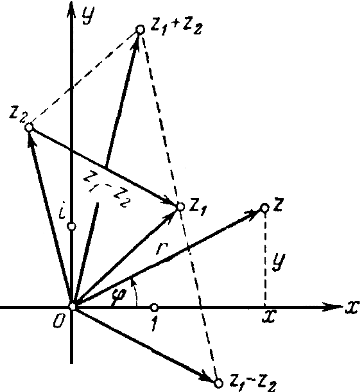
\includegraphics[width=.45\linewidth]{mal-01.png}
	\label{fig:1}
\end{figure}

З цього малюнку зрозумілий \textit{геометричний зміст} додавання і віднімання комплексних чисел. \\

Надалі наряду з представленням комплексних чисел у декартових координатах, корисно буде мати їх представлення у \textit{полярних} координатах. Для цього, як зазвичай, суміщаємо полярну вісь з додатною піввіссю $x$, а полюс -- з початком координат. \\

Тоді, якщо позначити через $r$ полярний \textit{радіус}, а через $\phi$ -- полярний \textit{кут} точки $z$, то будемо мати
\begin{equation}
	\label{eq:1.2.1}
	z = x + i y = r (\cos \phi + i \sin \phi).
\end{equation}

Полярний радіус $r$ називається \textit{модулем} комплексного числа $z$ і позначається символом $|z|$, кут $\phi$ -- його \textit{аргументом} і позначається символом $\Arg z$. \\

Модуль комплексного числа визначається \textit{однозначно}:
\begin{equation}
	\label{eq:1.2.2}
	|z| = \sqrt{x^2 + y^2} \ge 0,
\end{equation}
а його аргумент визначається \textit{з точністю до $2 k \pi$}:
\begin{equation}
	\label{eq:1.2.3}
	\phi = \Arg z = \begin{cases} \arctan \left(\dfrac yx\right) + 2 k \pi, & (\text{I та ІV квадранти}), \\ \\ \arctan \left(\dfrac yx\right) + (2 k + 1) \pi, & (\text{II i III квадранти}), \end{cases}
\end{equation}
де $\arctan$ позначає головне значення $\Arctan$, тобто таке, що належить $\left(-\frac\pi2,\frac\pi2\right]$, $k$ -- довільне ціле число. \\

Надалі, наряду з $\Arg z$ ми будемо використовувати символ $\arg z$ який буде позначати \textit{одне} зі значень $\Arg z$, здебільшого головне. \\

Виконуються наступні нерівності:
\begin{equation}
	\label{eq:1.2.4}
	|z_1 + z_2| \le |z_1| + |z_2|; \quad |z_1 - z_2| \ge ||z_1| - |z_2||.
\end{equation}
Причому рівність \textit{досягається} лише коли $\Arg z_1 = \Arg z_2$, або одне з чисел нуль. \\

З визначення \eqref{eq:1.1.8} попереднього пункту випливає, що при множенні комплексних чисел їх модулі \textit{множаться}, а їх аргументи \textit{додаються}. Справді,
\begin{multline}
	\label{eq:1.2.5}
	z_1 \cdot z_2 = r_1 \cdot r_2 ((\cos \phi_1 \cdot \cos\phi_2 - \sin \phi_1 \cdot \sin \phi_2) + \\
	+ i (\sin \phi_1 \cdot \cos \phi_2 + \sin \phi_2 \cdot \cos \phi_1)) = \\
	= r_1 \cdot r_2 (\cos (\phi_1 + \phi_2) + i \sin (\phi_1 + \phi_2)).
\end{multline}

Звідси випливає, що при множенні комплексного числа $z_1$ на $z_2$ вектор $z_1$ \textit{розтягується} в $|z_2|$ разів і повертається (проти годинникової стрілки) на кут $\arg z_2$. \\

Зокрема, множення комплексного числа $z$ на $i$ зводиться до повороту (без розтягнення) вектору $z$ на \textit{прямий} кут проти годинникової стрілки. \\

Для побудови добутку $z = z_1 \cdot z_2$ достатньо на відрізку $Oz_1$ як на основі побудувати трикутник $Oz_1z$ який \textit{подібний} трикутнику $Oz_1z_2$. \\

\begin{figure}[H]
	\centering
	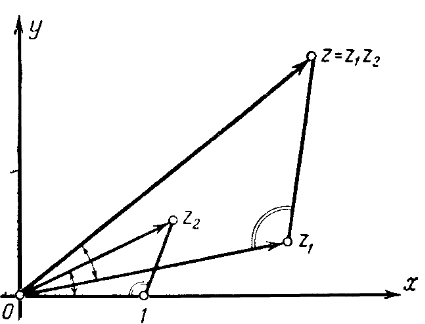
\includegraphics[width=.45\linewidth]{mal-02.png}
	\label{fig:2}
\end{figure}

Ділення комплексного числа $z_1$ на $z_2$ зводиться до множення $z_1$ на $1 / z_2$, тому достатньо з'ясувати геометричний зміст операції $w = 1 / z$. Нехай спершу $|z| < 1$:

\begin{figure}[H]
	\centering
	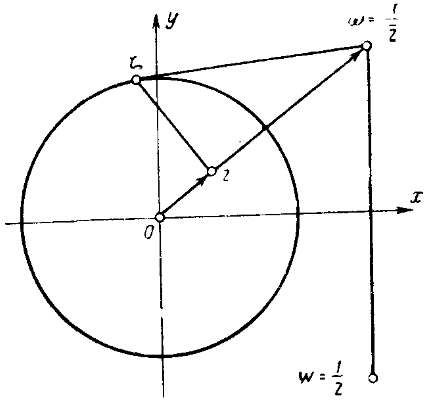
\includegraphics[width=.45\linewidth]{mal-03.png}
	\label{fig:3}
\end{figure}

Опустимо із точки $z$ перпендикуляр на промінь $Oz$ і через точку $\zeta$ перетину перпендикуляра із колом $|z| = 1$ проведемо \textit{дотичну} до цього кола. \\

Для точки $\omega$ перетину побудованої дотичної із променем $Oz$ маємо 
\begin{equation}
	\label{eq:1.2.6}
	\Arg \omega = \Arg z,
\end{equation}
а з подібності прямокутних трикутників $Oz\zeta$ і $O\zeta \omega$ маємо 
\begin{equation}
	\label{eq:1.2.7}
	|\omega| / |\zeta| = |\zeta| / |z|,
\end{equation}
\textit{звідки} $|\omega| = 1 / |z|$, адже $|\zeta| = 1$. \\

Таким чином, число $\omega$ є спряженим до числа $1 / z$, $\omega = 1 / \overline{z}$, і для отримання точки $w = 1 / z$ достатньо побудувати точку, \textit{симетричну} до точки $\omega$ відносно дійсної вісі. \\

Перехід від точки $z$ до точки $\omega = 1 / \overline{z}$ називається \textit{інверсією}, або \textit{симетрією відносно} одиничного \textit{кола} $|z| = 1$. \\

Таким чином, операція $w = 1 / z$ геометрично зводиться до \textit{двох послідовних симетрій} -- інверсії і симетрії відносно дійсної вісі. \\

Якщо ж $|z| > 1$ то описані побудови варто проводити у \textit{зворотному} порядку, а якщо $|z| = 1$, то точка $\omega = 1 / \overline{z}$ збігається з точкою $z$ і побудова $w = 1 / z$ зводиться до симетрії відносно дійсної вісі. \\

Геометричний сенс піднесення до степеня зрозумілий з геометричного сенсу множення. \\

Для побудови коренів степеню $n$ із $z$ помітимо, що із визначення кореня і формули \eqref{eq:1.2.5} для $w = \sqrt[n]{z}$ маємо 
\begin{equation}
	\label{eq:1.2.8}
	|w|^n = |z|, \quad n \arg w = \arg z,
\end{equation}
тому
\begin{equation}
	\label{eq:1.2.9}
	|w| = \sqrt[n]{z}, \quad \arg w = \dfrac{\arg z}{n}.
\end{equation}

Перше зі співвідношень \eqref{eq:1.2.9} показує, що модулі всіх коренів рівні, а друге -- що їх аргументи відрізняються на кратне $2 \pi / n$, бо до значення $\arg z$ можна додавати кратне $2 \pi$. \\

Звідси випливає, що корінь степеню $n$ із довільного комплексного числа $z \ne 0$ має $n$ \textit{різних} значень, і що це значення розташовані у вершинах правильного $n$-кутника вписаного у коло $|w| = \sqrt[n]{|z|}$:
\begin{figure}[H]
	\centering
	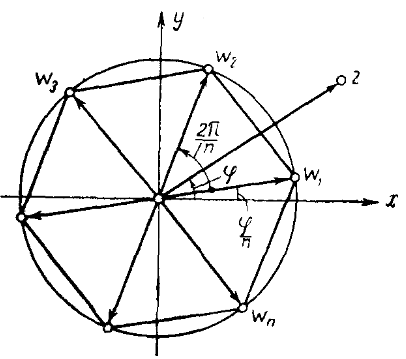
\includegraphics[width=.45\linewidth]{mal-04.png}
	\label{fig:4}
\end{figure}

% \flushright{\copyright \, М. А. Лаврентьев, Б. В. Шабат, 1972 \\ Українською переклав Нікіта Скибицький, 2018}

% \end{document}